\section{Tổ chức thư mục của chương trình}
Chương trình được tổ chức như sau.
Ở server:
\begin{figure}[H]
\centering{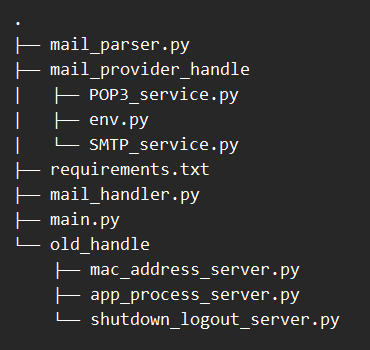
\includegraphics[scale=1]{server_dir}}
\caption{Tổ chức thư mục ở server}
\end{figure}
Server có thư mục \textbf{mail$\mathbf{\_}$provider$\mathbf{\_}$handle} chứa các module phục vụ cho quá trình gửi và nhận mail, thư mục \textbf{old$\mathbf{\_}$handle} chứa một vài hàm được cung cấp sẵn cho quá trình xử lý các yêu cầu. \\
Module \textbf{mail$\mathbf{\_}$parser.py} chứa hàm phục vụ cho quá trình phân tích lệnh được nhận từ email. Module \textbf{mail$\mathbf{\_}$handler} chứa các hàm xử lý yêu cầu, giao tiếp với client và trả kết quả. \\
Tập tin \textbf{requirements.txt} chứa các yêu cầu cần thiết (bên cạnh Python 3.9 trở lên) để chạy chương trình.\\
Tập tin \textbf{main.py} là tập tin chính của server, ta cần chạy tập tin này để khởi động server. \textbf{Lưu ý} khi chạy tập tin này, ta cần thay đổi giá trị \textbf{MAX$\mathbf{\_}$CONNECTION} ở dòng 13 thành giá trị \textbf{bằng đúng} với số lượng client (tối đa 4).
Ở client:
\begin{figure}[H]
\centering{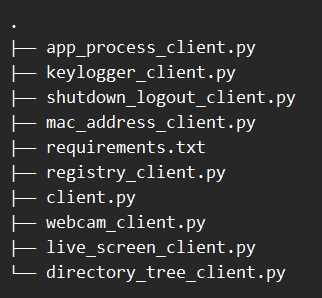
\includegraphics[scale=1]{victim_dir}}
\caption{Tổ chức thư mục ở client}
\end{figure}
Tập tin \textbf{requirements.txt} chứa các yêu cầu cần thiết (bên cạnh Python 3.9 trở lên) để chạy chương trình.\\
Trừ tập tin \textbf{client.py}, các tập tin mã nguồn Python còn lại chứa các hàm xử lý các yêu cầu được gửi đến từ server.\\
Tập tin \textbf{client} là tập tin chính của client, ta cần chạy tập tin này để khởi động client. \textbf{Lưu ý} khi chạy tập tin này ta cần thay đổi giá trị 127.0.0.1 ở dòng 60 thành một giá trị thích hợp.\\
\textbf{Tất cả các client phải được kết nối đến server TRƯỚC khi server bắt đầu nhận và xử lý các lệnh từ email.}

